\chapter*{Introduction}
\addcontentsline{toc}{chapter}{Introduction}
	\par \textbf{Survive} is a take on the game \textbf{Survive - Wilderness survival}\cite{Survive} by \textbf{Juuso Hietalahti}\cite{Juuso}.

	\section*{Motivation}
	\addcontentsline{toc}{section}{Motivation}
		\par My favourite \textbf{programming direction} discovered in University has been \textbf{game development}. As an avid \textbf{lifelong player}, I have always brushed away the idea of \textbf{pursuing} it as more than a \textbf{hobby}. The practice is still quite \textbf{uncommon} in the \textbf{courses} and \textbf{career paths} found in Romania. 
		\par Throughout \textbf{college}, I managed to obtain some sort of \textbf{game system assignment} for the majority of the \textbf{mandatory projects} I had. The \textbf{Game Design}\cite{Course} course created by my \textbf{coordinator} was the reason I finally decided to take it seriously and choose a \textbf{game} for my \textbf{Bachelor's Thesis}.
		\par My favourite games belong to the \textbf{survival, strategy} and \textbf{simulation} genres. I have been playing \textbf{Survive - Wilderness survival} for many years, even though I enjoy \textbf{PC games} much more.  My \textbf{interest} and its \textbf{complexity} made it an \textbf{attainable, good choice} for my \textbf{Thesis}. 


	\section*{Gameplay Description}
	\addcontentsline{toc}{section}{Gameplay Description}
		\par \textbf{Survive} a long, challenging, resource-scarce \textbf{journey} back to the main road after getting lost in the woods on a rainy day. \textbf{Forage} for wood, berries, water and vines. \textbf{Hunt, fish, rest, cook} and \textbf{craft} campfires, weapons, traps, bandages and clothing insulators.
    	\par \textbf{Travel}, take different turns and make \textbf{strategic} choices in order to reach civilization before it is too late. Balance \textbf{hunger, temperature, thirst, health} and inventory to avoid \textbf{starvation, hypothermia, dehydration and illness}.
    	\par Stay alive or \textbf{permanently lose} the game and start over!

	\section*{Requirements}
	\addcontentsline{toc}{section}{Requirements}
		\par The \textbf{project} must be an \textbf{Android} application with an interface that recognizes \textbf{one finger screen touch}. It should be easy to \textbf{download} and to \textbf{install} on a \textbf{mobile device}. 
		\par The \textbf{player} should be allowed to \textbf{pause, resume, save} and \textbf{quit} the game quickly. \textbf{Exiting} has to lead to \textbf{discarding} unsaved \textbf{progress} and \textbf{dying} must result in a \textbf{game over}, as one of the main design characteristics is \textbf{permanent death}(the player loses for good, \textbf{no second chances}). 
		\par The \textbf{project} must offer the \textbf{medium difficulty gameplay} with the original \textbf{objective}: \textbf{surviving} a long track back to a main road after getting lost in the woods. The \textbf{mechanics} ought to include \textbf{sleeping, crafting, item manipulation, collecting resources, travel, fire starting} and \textbf{traps}. The \textbf{time progression, status bars} and \textbf{items} should be relatively \textbf{similar} to the original.

	\section*{Approach}
	\addcontentsline{toc}{section}{Approach}
		\par I chose to \textbf{implement} the game using \textbf{Python}, as I am very comfortable with it. 
		\par I tried to use \textbf{PyGame}\cite{Pygame} for the \textbf{GUI}, until I realized that it is not suited for \textbf{mobile applications}, so I switched the progress to \textbf{Kivy}\cite{Kivy}, a cross-platform Python framework.
		\par I approached \textbf{loading/saving} with the Python module \textbf{Pickle}\cite{Pickle} and the Android \textbf{executable} was made with \textbf{Buildozer}\cite{Buildozer}. 

	\section*{Related Work}
	\addcontentsline{toc}{section}{Related Work}
	\par \textbf{Survive - Wilderness survival}\cite{Survive}(\textit{Fig.(a)}) is a \textbf{mobile game} originally developed by \textbf{Juuso Hietalahti}\cite{Juuso}. It has more than \underline{5} \textbf{million downloads} and a \underline{4} \textbf{star rating} from over \underline{127.000} people. The main genre is \textbf{Survival}, mixed with \textbf{Strategy, Crafting} and \textbf{Simulation}. It has an \textbf{age restriction} for people under \underline{10} years old. The engine used is \textbf{Unity} and the language is \textbf{C\#}. 
		\begin{figure}[H]
			\centering
			\subfigure[\textbf{App Store Game Banner}]{\label{fig:a}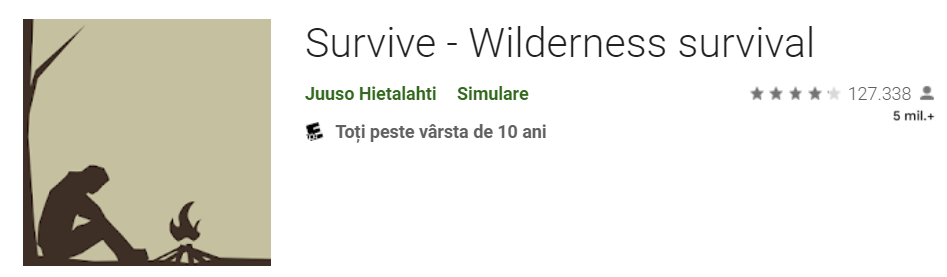
\includegraphics[width=15cm, height=5cm]{Images/OriginalBanner.png}}
		\end{figure}
		\par \textbf{Juuso Hietalathi}\cite{Juuso} is a \textbf{game developer} from \textbf{Finnland}. He started working on the project during a \underline{24} hour \textbf{Game Design Contest}, where he \textbf{won first place} for his \textbf{idea} and \textbf{rough implementation}. It was so successful that he \textbf{continued development} with the intention of \textbf{selling} it. Many years later, the \textbf{game}(\textit{Fig.(b)}) has \textbf{millions of downloads} and there is an \textbf{Android} and \textbf{iOS remake} in the works.
		\begin{figure}[H]
			\centering
			\subfigure[\textbf{App Store Game Cover}]{\label{fig:b}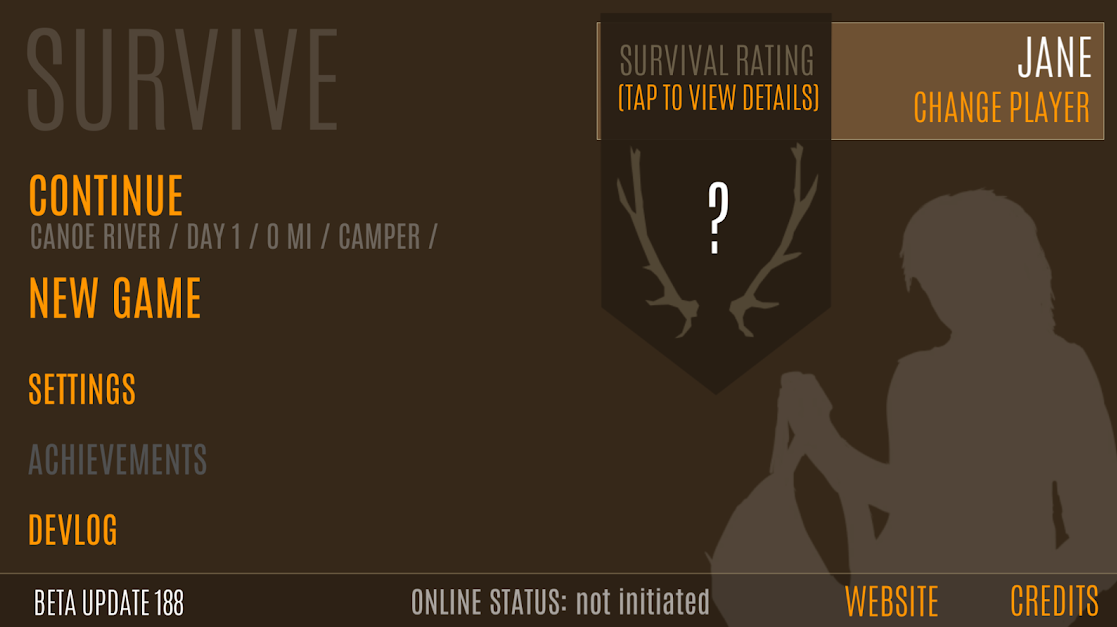
\includegraphics[width=10cm, height=5cm]{Images/OriginalCover.png}}
		\end{figure}
\newpage


\chapter*{Contribution}
\addcontentsline{toc}{chapter}{Contribution}
	\par The \textbf{thought process} leading to my \textbf{choice of project} contained many questions and requirements. It had to be a \textbf{game} in my favourite genres, \textbf{reasonable to implement} in one \textbf{semester} and full of \textbf{learning} potential.
	\par My decision, \textbf{"Survive - Wilderness survival"} turned out to have many \textbf{positives}. Almost \textbf{everything} is \textbf{new to me} in terms of implementation: the \textbf{platform}, the \textbf{genres}, the \textbf{gameplay}. I have never made an \textbf{Android Application} before, so I got to \textbf{experiment} with many new routes of \textbf{game} design and development. It was very \textbf{versatile} in terms of \textbf{languages} and \textbf{game engines}, so I could choose to be as \textbf{comfortable} or as \textbf{challenged} as I wanted to be.
	\par This \textbf{game} is \textbf{not new} to me. I \textbf{played} it before, it's the simplest \textbf{survival game} I have ever enjoyed. I had \textbf{tester insight}, I got to be the \textbf{target audience} for the project I was implementing. My \textbf{contribution} to the concept can be found in all the \textbf{differences} between the \textbf{original} and \textbf{my} development \textbf{journeys}. 

	\section*{Time Frame}
	\addcontentsline{toc}{section}{Time Frame}
		\par I did not spend \textbf{two years} designing a game from \textbf{scratch}, I spent \textbf{three months} \textbf{guessing} the steps someone else made, \textbf{analysing} why they made them and why they \textbf{succeeded}. I had a lot \textbf{less time} to complete a different set o \textbf{tasks}.

	\section*{Design Stages}
	\addcontentsline{toc}{section}{Design Stages}
		\par My \textbf{design decisions} were made as a result of a \textbf{two-step process}. \textbf{Replaying} the original game as many times as possible in order to \textbf{gather data} and guess what values were originally used, and \textbf{comparing} it to what I could or what I would rather \textbf{prefer} doing. 

	\section*{Technologies}
	\addcontentsline{toc}{section}{Technologies}
		\par The \textbf{original game} is implemented in \textbf{Unity}(a game engine) with \textbf{C\#}. I used \textbf{Python} and a \textbf{library}, leaving me a lot of \textbf{GUI elements} to make from \textbf{scratch}. This helped me a lot in my goal to \textbf{learn} as much as possible about the \textbf{basics}. \\ \\


	\par The \textbf{original} developer \textbf{designed} a game from \textbf{scratch}, with an \textbf{engine} that allowed a lot of freedom and \textbf{readily} implemented code, in the span of \textbf{2 years}. I took the role of \textbf{data analyst, tester, target audience} and \textbf{core back-end programmer} for \textbf{three months}, in a \textbf{different language}.

\newpage


